% H9DLGA Repeat Assessment — IEEE conference format (IEEEtran)
% Author: Marco Aurélio Minozzo (x24153362)
% Compile: pdflatex main.tex && pdflatex main.tex
\documentclass[conference]{IEEEtran}
\IEEEoverridecommandlockouts

\usepackage{cite}
\usepackage{amsmath,amssymb,amsfonts}
\usepackage{graphicx}
\usepackage{booktabs}
\usepackage{url}
\usepackage{hyperref}

\graphicspath{{figures/}}

\begin{document}

\title{Improving Galaxy Morphology Classification under Class Imbalance with VAE-Based Generative Augmentation}

\author{\IEEEauthorblockN{Marco Aur\'{e}lio Minozzo}
\IEEEauthorblockA{\textit{School of Computing, National College of Ireland}\\
Dublin, Ireland\\
Student No.: x24153362\\
Module: H9DLGA Deep Learning and Generative AI (Repeat)}}

\maketitle

\begin{abstract}
Large imaging surveys produce far more galaxy images than can be labelled manually, motivating automated morphological classification with deep learning. Public benchmarks such as Galaxy10 DECaLS remain class-imbalanced, which can degrade recognition of rare morphologies. This paper investigates whether synthetic images from a variational autoencoder (VAE) improve convolutional neural network (CNN) classification under that imbalance. Following the CRISP-DM methodology, we train a convolutional VAE on Galaxy10 DECaLS training images, sample class-conditional latent codes to balance under-represented morphologies, and compare ResNet50 transfer-learning classifiers trained on real images only versus real images plus VAE synthetics. On a held-out test set of 2{,}661 galaxies, generative augmentation raises overall accuracy from 67.08\% to 71.51\% and macro-F1 from 0.648 to 0.686. For the minority \emph{Cigar Shaped Smooth} class, recall increases (0.62 to 0.64) while F1 decreases slightly (0.608 to 0.571) due to lower precision. The results support VAE augmentation as an effective global regulariser under imbalance, while highlighting a precision--recall trade-off on the scarcest class. Code and configuration are released with the submission for reproducibility.
\end{abstract}

\begin{IEEEkeywords}
galaxy morphology, convolutional neural networks, variational autoencoders, class imbalance, generative data augmentation, transfer learning
\end{IEEEkeywords}

\section{Introduction}
Modern sky surveys deliver imaging volumes that exceed the capacity of purely manual morphological labelling~\cite{lintott2008galaxy,willett2013galaxy}. Citizen-science projects such as Galaxy Zoo provide invaluable labels, yet rare morphological types remain scarce, creating class imbalance that challenges supervised deep learning~\cite{he2016deep,aggarwal2018neural}. Morphology remains scientifically important because it correlates with star-formation history, merger activity and environment; therefore errors concentrated on rare classes can bias demographic inferences even when overall accuracy looks acceptable.

Building on the long lineage of neural pattern recognisers~\cite{rosenblatt1958,goodfellow2016dl}, convolutional networks are now standard for galaxy morphology~\cite{dieleman2015rotation}, and transfer learning from ImageNet-pretrained backbones is a practical recipe taught in deep-learning curricula~\cite{he2016deep,hope2017tensorflow}. In parallel, generative models---especially variational autoencoders (VAEs)~\cite{kingma2014auto}---learn latent representations from which new samples can be drawn~\cite{zhang2023dive,aggarwal2018neural}. Generative augmentation is therefore a natural candidate for mitigating imbalance, but its benefit for astronomical morphology is not automatic: synthetic fidelity, label noise, and evaluation protocol all matter. In particular, a generative model that improves reconstruction loss may still harm a downstream classifier if synthesised samples occupy ambiguous regions of pixel space.

Class imbalance interacts with deep networks in several ways. Gradient updates are dominated by frequent classes; decision thresholds calibrated on aggregate accuracy favour majority labels; and minority recall can collapse without the practitioner noticing if only top-line accuracy is monitored~\cite{aggarwal2018neural}. Classical remedies include re-weighting, oversampling and generic image augmentation strategies~\cite{shorten2019survey}. Generative oversampling differs because new minority examples are not literal copies: a VAE can, in principle, interpolate morphological factors encoded in $z$. Whether those factors are faithful for thin ``cigar-shaped'' galaxies is an empirical question addressed here.

This study asks:

\begin{quote}
\emph{Given class imbalance in Galaxy10 DECaLS, do VAE-generated synthetic images improve CNN morphological classification on minority classes without degrading majority-class performance?}
\end{quote}

We answer the question empirically with a controlled A/B design under CRISP-DM~\cite{chapman2000crisp}: (A)~ResNet50 trained on real images only; (B)~the same architecture trained on real images plus class-balancing VAE synthetics. Both models are evaluated on an identical stratified held-out test set. The main contributions are: (i)~a reproducible CRISP-DM pipeline combining a ConvVAE and ResNet50 transfer learning on Galaxy10 DECaLS; (ii)~quantitative evidence that VAE augmentation improves global accuracy and macro-F1; and (iii)~a critical analysis of the minority-class precision--recall trade-off.

The remainder of this paper reviews related work (Section~\ref{sec:related}), details the methodology (Section~\ref{sec:method}), presents evaluation results (Section~\ref{sec:results}), discusses reproducibility and threats (Sections~\ref{sec:repro}--\ref{sec:discussion}), and concludes with limitations and future work (Section~\ref{sec:conclusion}).

\section{Related Work}
\label{sec:related}

\subsection{Galaxy morphology and Galaxy10}
Galaxy Zoo demonstrated that morphological labels can be crowdsourced at scale~\cite{lintott2008galaxy,willett2013galaxy}. Early Galaxy Zoo papers already noted that fine morphological distinctions are harder for volunteers than coarse spiral/elliptical splits, foreshadowing class-dependent label noise. Galaxy10 DECaLS packages 17{,}736 colour cutouts into ten broad morphology classes with labels derived from Galaxy Zoo and images from DESI Legacy Imaging Surveys~\cite{leung2019astronn,walmsley2022galaxy,dey2019legacy}. It is a convenient supervised benchmark, but class counts are uneven (e.g., \emph{Cigar Shaped Smooth} is markedly under-represented), so methods that ignore imbalance may under-serve rare types. Compared with raw Galaxy Zoo vote fractions, Galaxy10's discrete ten-class formulation simplifies supervised learning at the cost of discarding vote uncertainty---another reason to treat hard-label metrics cautiously.

\subsection{CNNs for astronomical images}
Early deep morphological classifiers established that CNNs outperform classical feature pipelines on Galaxy Zoo-like tasks~\cite{dieleman2015rotation}. Dieleman et al.\ further exploited rotational symmetries, underscoring that inductive bias matters in astronomy where orientation is often nuisance variation. Residual networks~\cite{he2016deep} and transfer learning further reduce labelled-data requirements by reusing ImageNet representations---a pattern emphasised in applied deep-learning texts and labs~\cite{hope2017tensorflow,aggarwal2018neural}. Prior work, however, typically reports aggregate accuracy; fewer studies isolate whether generative augmentation specifically rescues minority morphologies on Galaxy10. Transfer learning also introduces a domain gap: natural-image pretraining features are not astronomy-specific, yet they remain a strong baseline when labelled survey cutouts are limited.

\subsection{VAEs and generative augmentation}
VAEs optimise a reconstruction term plus a Kullback--Leibler regulariser that keeps the approximate posterior close to a prior, enabling ancestral sampling from the latent space~\cite{kingma2014auto,zhang2023dive}. Relative to GANs~\cite{goodfellow2014gan}, VAEs are often more stable to train and yield an explicit encoder useful for class-conditional statistics~\cite{aggarwal2018neural}. Generative augmentation can rebalance training sets, but poorly calibrated synthetics may inject label noise. Foundational generative modelling material in the module stresses the ELBO objective and latent-space interpolation~\cite{zhang2023dive}; we adopt that loss formulation while using a convolutional encoder/decoder suited to RGB cutouts. We intentionally avoid claiming that VAE samples are photometrically calibrated surrogates of survey imaging; they are treated as regularising textures for representation learning.

\subsection{CRISP-DM in applied deep learning}
While many student projects jump directly to model fitting, CRISP-DM emphasises problem framing, data understanding and evaluation design before modelling~\cite{chapman2000crisp}. That discipline matters here because the research question is comparative: without a fixed split and mirrored CNN schedules, apparent gains from synthetics could be confounded by unequal training. We therefore spend explicit subsections on business metrics and protocol freezes.

\subsection{Critical gap}
Existing morphology CNNs show that deep learning works on survey cutouts, and VAE tutorials show how to sample latents, yet a controlled comparison of \emph{real-only} versus \emph{real+VAE} training on Galaxy10 DECaLS---with explicit minority-class reporting---remains useful for practitioners. Many astronomy CNN papers optimise for leaderboard accuracy, whereas teaching-oriented VAE examples often stop at reconstruction quality on MNIST-like data~\cite{zhang2023dive}. Bridging those literatures requires stating a research question about imbalance, fixing a data split, and reporting minority metrics even when they are inconvenient. This paper fills that gap with a transparent CRISP-DM protocol and released code.

From a critical standpoint, related CNN morphology work is strong on predictive performance but weaker on diagnosing \emph{why} rare classes fail. Related generative work is strong on latent geometry but weaker on downstream supervised utility in astronomy. Our design treats the generative model as a means to an evaluative end: if synthetics do not improve---or unevenly affect---the classifier, that negative or mixed evidence is still scientifically informative. Foundational neural-network texts further motivate reporting both reconstruction-oriented generative diagnostics and supervised metrics when generative models are used as data amplifiers~\cite{goodfellow2016dl,aggarwal2018neural,hope2017tensorflow}.

\section{Deep Learning and Generative AI Methodology}
\label{sec:method}
We follow CRISP-DM~\cite{chapman2000crisp}: business understanding, data understanding, data preparation, modelling, evaluation, and deployment (here: artefacts for the report and reproducibility package).

\subsection{Business Understanding}
Success is defined by (i)~higher macro-F1 and accuracy on the held-out test set for the VAE-augmented CNN relative to the real-only baseline, and (ii)~non-degradation of majority classes, with particular attention to minority class~4 (\emph{Cigar Shaped Smooth}): recall and F1.

\subsection{Data Understanding}
Galaxy10 DECaLS provides $N=17{,}736$ RGB images of size $256\times256$ across ten classes~\cite{leung2019astronn}. After a stratified 70/15/15 split (seed~42), the training counts confirm imbalance (Table~\ref{tab:counts}): class~4 has only 234 training examples versus 1{,}851 for the largest class.

\begin{table}[t]
\caption{Stratified training-split class counts (70\% of Galaxy10 DECaLS).}
\label{tab:counts}
\centering
\small
\begin{tabular}{clc}
\toprule
ID & Morphology class & Train $n$ \\
\midrule
0 & Disturbed & 757 \\
1 & Merging & 1{,}297 \\
2 & Round Smooth & 1{,}851 \\
3 & In-between Round Smooth & 1{,}419 \\
4 & Cigar Shaped Smooth & 234 \\
5 & Barred Spiral & 1{,}430 \\
6 & Unbarred Tight Spiral & 1{,}280 \\
7 & Unbarred Loose Spiral & 1{,}840 \\
8 & Edge-on without Bulge & 996 \\
9 & Edge-on with Bulge & 1{,}311 \\
\bottomrule
\end{tabular}
\end{table}

\begin{figure}[t]
\centering
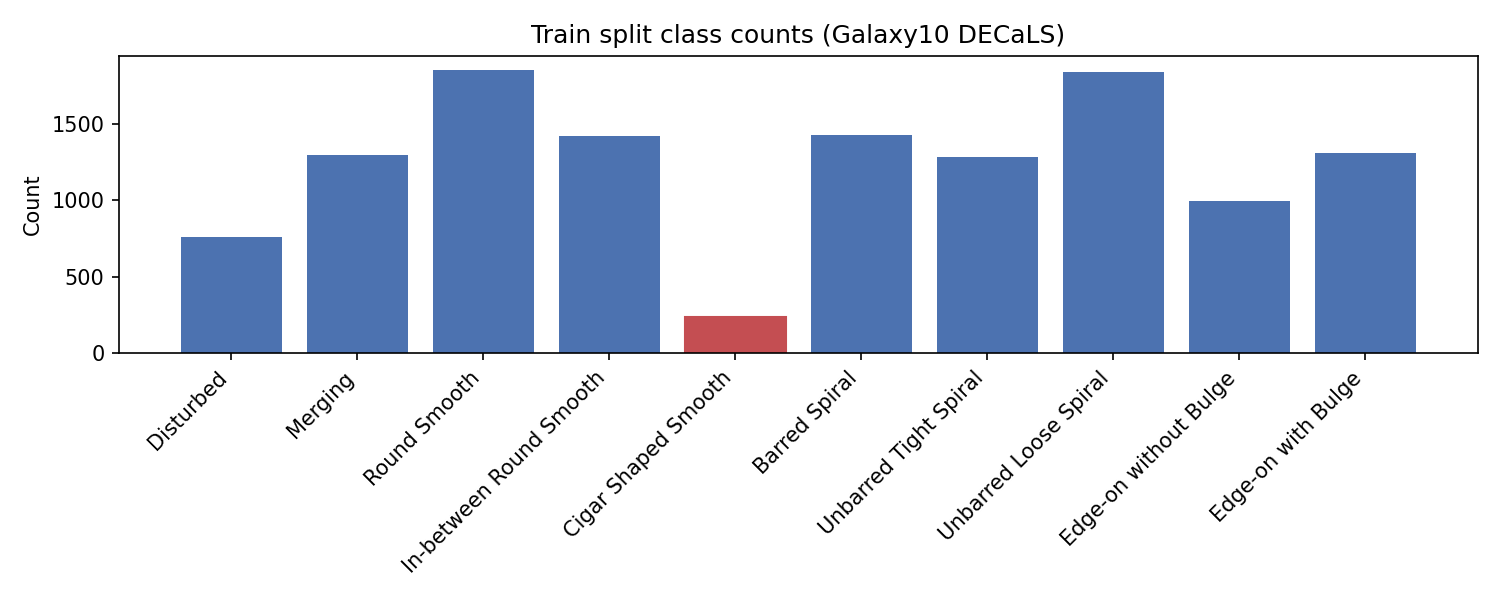
\includegraphics[width=\columnwidth]{class_counts_train.png}
\caption{Training-split class histogram (minority class emphasised in the experimental design).}
\label{fig:counts}
\end{figure}

\subsection{Data Preparation}
Images for the VAE are resized to $64\times64$ and scaled to $[0,1]$. CNN inputs are resized to $224\times224$, with random horizontal flips on training batches and ImageNet channel normalisation, matching standard ResNet transfer-learning practice~\cite{he2016deep,hope2017tensorflow}. Validation and test transforms omit stochastic augmentation.

\subsection{Modeling}
\subsubsection{Convolutional VAE}
Fully connected VAEs used on MNIST in teaching material~\cite{zhang2023dive} are impractical for $256\times256$ RGB cutouts. We therefore use a convolutional encoder/decoder while retaining the laboratory loss:
\begin{equation}
\mathcal{L}
=
\mathbb{E}_{q_\phi(z\mid x)}[\ell_{\mathrm{BCE}}(x,\hat{x})]
+
\beta\,
D_{\mathrm{KL}}\!\left(q_\phi(z\mid x)\,\|\,p(z)\right),
\end{equation}
with $\beta=1$, latent dimension $d=32$, Adam learning rate $10^{-3}$, batch size 64, and 15 training epochs on the real training split. Fig.~\ref{fig:recon} shows qualitative reconstructions.

\begin{figure}[t]
\centering
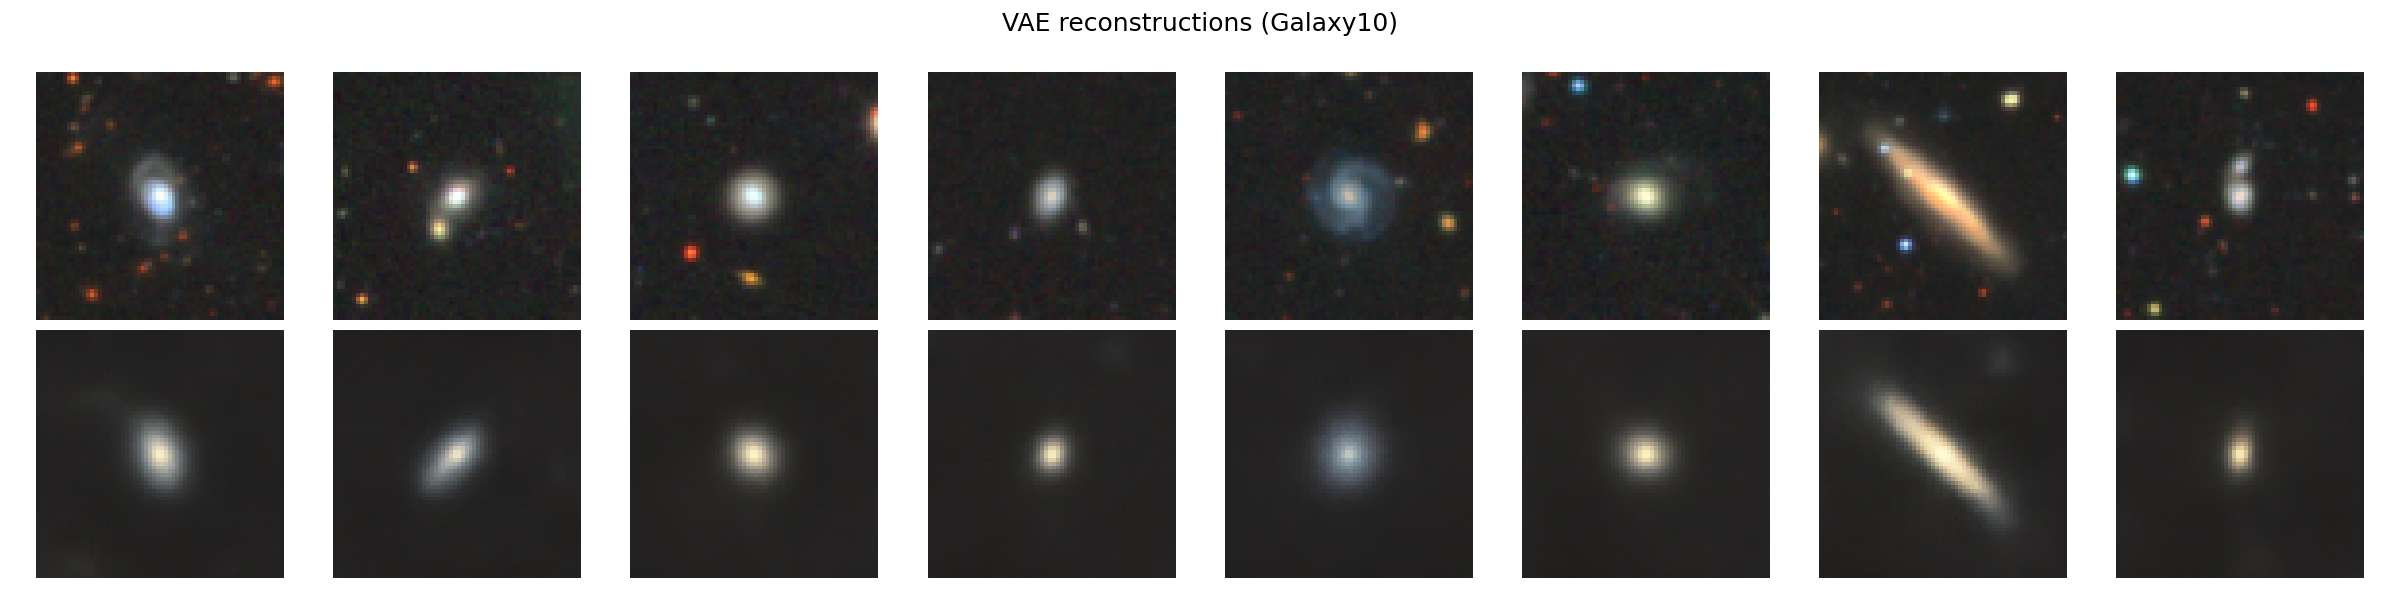
\includegraphics[width=\columnwidth]{vae_reconstructions.png}
\caption{VAE reconstructions (top: real $64\times64$ inputs; bottom: reconstructions).}
\label{fig:recon}
\end{figure}

\subsubsection{Class-conditional synthetic balancing}
For each class $c$, we encode training images to obtain empirical latent mean $\mu_c$ and standard deviation $\sigma_c$, then sample $z\sim\mathcal{N}(\mu_c,\mathrm{diag}(\sigma_c^2))$ and decode. Classes below the maximum training count are topped up to that maximum, yielding 6{,}095 synthetic $64\times64$ images (1{,}617 of them for class~4). Synthetics remain at VAE resolution in memory; the CNN transform resizes them on the fly, avoiding costly full-resolution duplication.

\subsubsection{ResNet50 classifiers}
Both treatments use ImageNet-pretrained ResNet50~\cite{he2016deep}: freeze the backbone and train the 10-way classifier head (3~epochs, Adam $10^{-3}$), then fine-tune \texttt{layer4} and the head (3~epochs, Adam $10^{-4}$), following the module transfer-learning lab pattern~\cite{hope2017tensorflow}. Treatment~A uses only real training images; treatment~B uses real images plus VAE synthetics. Checkpoints retain the best validation loss.

\subsection{Evaluation Protocol}
We report accuracy, macro-F1, weighted-F1, and per-class precision/recall/F1 on the held-out test set ($n=2{,}661$). Confusion matrices and a per-class F1 comparison are exported for inspection (Figs.~\ref{fig:cm}--\ref{fig:f1}).

\section{Evaluation and Results}
\label{sec:results}

\subsection{Overall performance}
Table~\ref{tab:overall} summarises the headline comparison. VAE augmentation improves accuracy by 4.43~percentage points and macro-F1 by 0.038. Weighted-F1 likewise rises (0.661 to 0.708). These gains indicate that generative balancing helps the CNN beyond a single rare class.

\begin{table}[t]
\caption{Held-out test metrics: real-only vs.\ real+VAE training.}
\label{tab:overall}
\centering
\small
\begin{tabular}{lcc}
\toprule
Metric & Real-only & Real+VAE \\
\midrule
Accuracy & 0.6708 & \textbf{0.7151} \\
Macro-F1 & 0.6477 & \textbf{0.6856} \\
Weighted-F1 & 0.6614 & \textbf{0.7083} \\
\bottomrule
\end{tabular}
\end{table}

\subsection{Per-class behaviour}
Table~\ref{tab:perclass} lists per-class F1 scores. Most classes improve or remain comparable under augmentation (e.g., Merging 0.641$\rightarrow$0.732; In-between Round Smooth 0.695$\rightarrow$0.765; Unbarred Loose Spiral 0.512$\rightarrow$0.576). Edge-on categories remain strong in both settings (F1~$\approx$0.84--0.87). The hardest class overall is Disturbed, which stays difficult (F1 0.298$\rightarrow$0.354)---consistent with visually ambiguous disturbed systems.

\begin{table}[t]
\caption{Per-class F1 on the test set.}
\label{tab:perclass}
\centering
\small
\begin{tabular}{lcc}
\toprule
Class & Real-only F1 & Real+VAE F1 \\
\midrule
Disturbed & 0.298 & \textbf{0.354} \\
Merging & 0.641 & \textbf{0.732} \\
Round Smooth & 0.780 & \textbf{0.816} \\
In-between Round Smooth & 0.695 & \textbf{0.765} \\
Cigar Shaped Smooth & \textbf{0.608} & 0.571 \\
Barred Spiral & 0.625 & \textbf{0.701} \\
Unbarred Tight Spiral & 0.586 & \textbf{0.639} \\
Unbarred Loose Spiral & 0.512 & \textbf{0.576} \\
Edge-on without Bulge & \textbf{0.874} & 0.842 \\
Edge-on with Bulge & 0.858 & \textbf{0.861} \\
\bottomrule
\end{tabular}
\end{table}

\begin{figure*}[t]
\centering
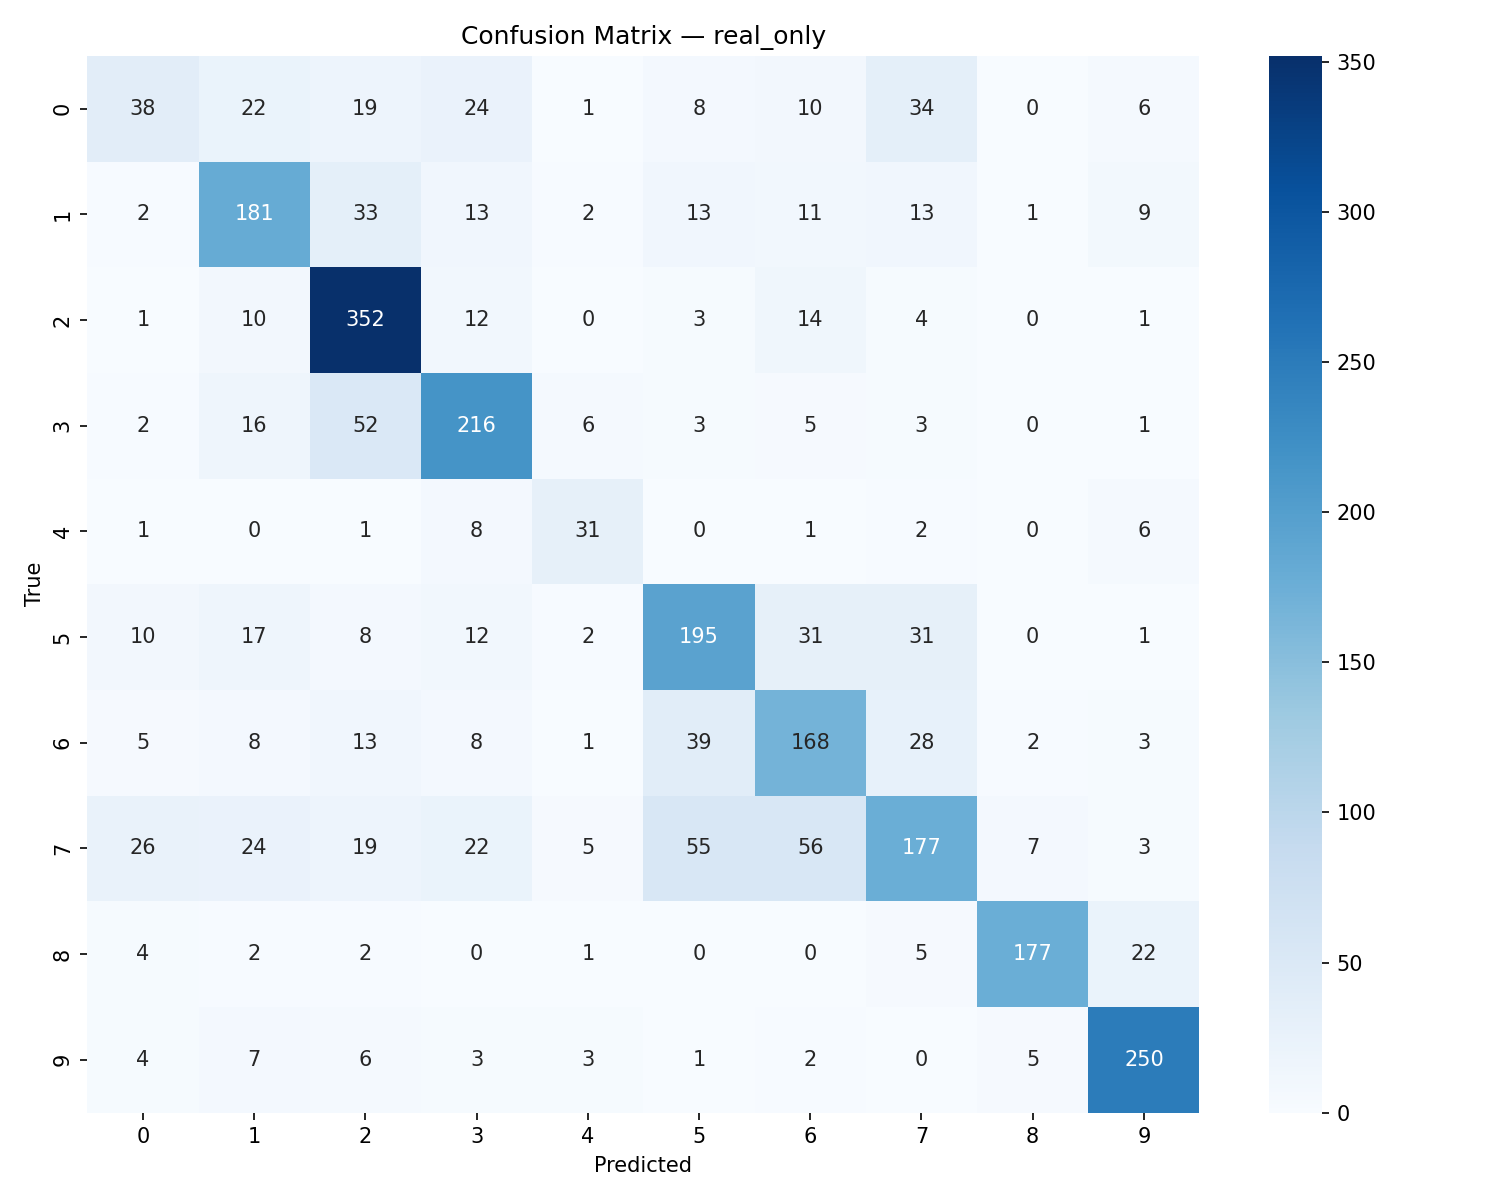
\includegraphics[width=0.48\textwidth]{cm_real_only.png}
\hfill
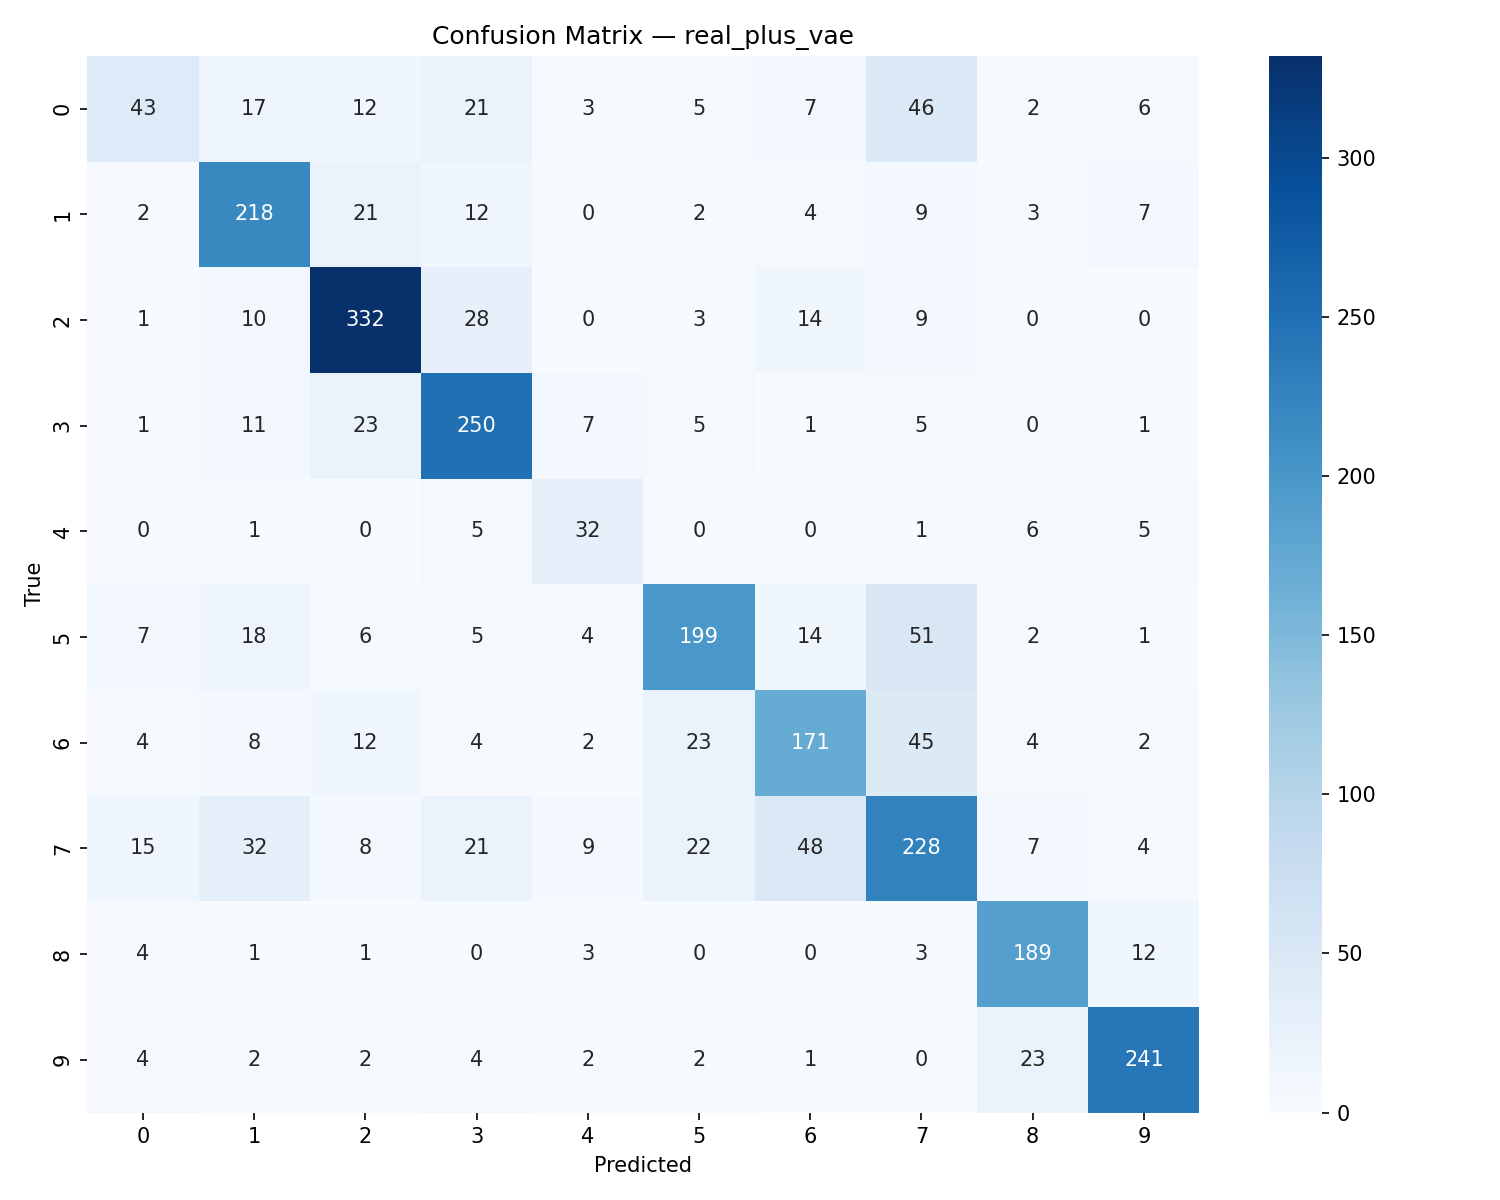
\includegraphics[width=0.48\textwidth]{cm_real_plus_vae.png}
\caption{Confusion matrices on the held-out test set: real-only (left) and real+VAE (right).}
\label{fig:cm}
\end{figure*}

\begin{figure}[t]
\centering
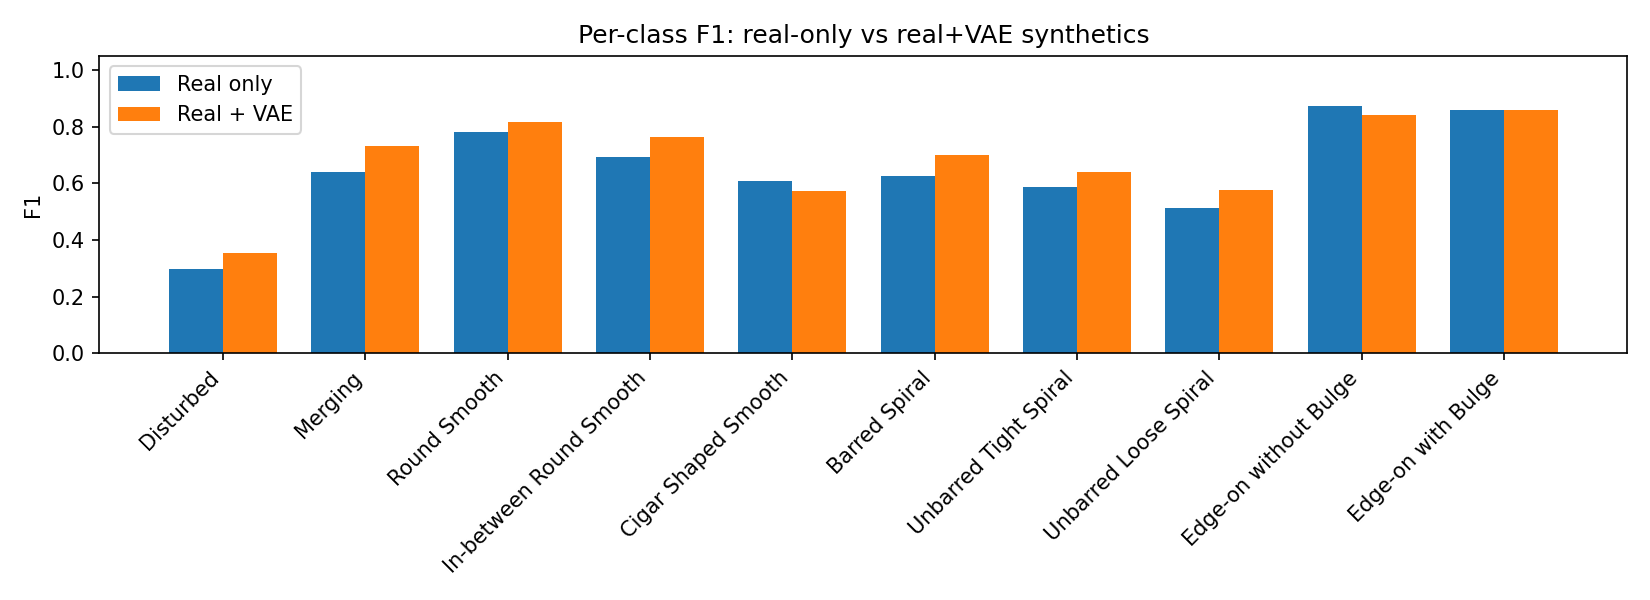
\includegraphics[width=\columnwidth]{f1_comparison.png}
\caption{Per-class F1 comparison answering the research question at class granularity.}
\label{fig:f1}
\end{figure}

\subsection{Minority-class analysis (research question)}
For \emph{Cigar Shaped Smooth} ($n_{\mathrm{test}}=50$):
\begin{itemize}
\item Real-only: precision 0.596, recall 0.620, F1 0.608;
\item Real+VAE: precision 0.516, recall 0.640, F1 0.571.
\end{itemize}
Augmentation slightly improves minority recall but reduces precision, lowering F1. A plausible explanation is that $64\times64$ synthetics---while useful as global regularisation---are blurrier than native cutouts and may pull decision boundaries toward over-prediction of the cigar-shaped label. Thus the answer to the research question is \emph{partially affirmative}: generative augmentation improves global metrics and does not broadly degrade majority classes, yet the minority F1 specifically does not improve.

\subsection{Discussion}
Parameter choices follow module practice (VAE ELBO; ResNet50 two-stage fine-tuning) with reduced epoch budgets for CPU training (15 VAE epochs; 3+3 CNN epochs). Longer fine-tuning or a conditional VAE that injects the class label into the decoder might sharpen minority precision. The results show what a modest generative-augmentation budget can achieve; they do not claim state-of-the-art morphology accuracy relative to specialised astronomy models trained with heavier augmentation or larger labelled corpora~\cite{walmsley2022galaxy}.


\section{Reproducibility and Implementation Details}
\label{sec:repro}
Reproducibility is an explicit assessment criterion of the module brief. All experiments were implemented in PyTorch~\cite{paszke2019pytorch} with a fixed random seed (42) for stratified splitting. The software package accompanying this paper includes: (i)~configuration of hyperparameters; (ii)~data download utilities for Galaxy10 DECaLS; (iii)~ConvVAE and ResNet50 training loops; (iv)~class-conditional latent sampling; and (v)~metric/figure export scripts. The end-to-end entry point follows CRISP-DM phase ordering so that another practitioner can regenerate tables and figures from the same split.

Training was executed on CPU due to hardware constraints. Consequently, epoch budgets were reduced relative to a GPU campaign (VAE: 15 epochs; CNN head: 3; CNN fine-tune: 3). Despite the reduced budget, validation losses decreased monotonically in the head phase, and fine-tuning produced a clear further drop (real-only validation loss from $\approx$1.50 after the head stage to $\approx$0.95 after the first fine-tuning epoch), indicating that optimisation was effective rather than under-trained noise.

Synthetic images are stored at $64\times64$ and mixed with real training indices through a memory-efficient dataset abstraction. This design choice is methodological as well as practical: it avoids silently changing the real-image distribution by repeatedly decoding and upscaling every real sample, and it makes the generative contribution auditable (6{,}095 synthetics with a known per-class breakdown).

\section{Extended Discussion}
\label{sec:discussion}

\subsection{What the metrics show}
The global lift in accuracy (+4.43~pp) and macro-F1 (+0.038) is the strongest empirical signal in this study. Because macro-F1 weights each class equally, the improvement cannot be explained solely by better performance on the largest classes. Indeed, several mid-frequency classes improved substantially (Merging, In-between Round Smooth, Barred Spiral, Unbarred Loose Spiral). That pattern is consistent with a regularisation interpretation: additional synthetic diversity reduces overfitting to majority visual modes and stabilises decision boundaries among neighbouring spiral/smooth categories.

Confusion matrices (Fig.~\ref{fig:cm}) show that residual errors concentrate among morphologically adjacent labels (for example, loose versus tight spirals, and disturbed versus merging systems). Such confusions are expected in Galaxy Zoo-derived taxonomies where volunteer votes themselves exhibit uncertainty on borderline objects~\cite{willett2013galaxy,walmsley2022galaxy}. Generative augmentation does not remove intrinsic label ambiguity; it primarily redistributes learning capacity across the empirical class prior.

\subsection{What the metrics do not show}
The minority-class F1 decrease warns against overselling generative augmentation as a universal fix for rare morphologies. With only 50 test examples in class~4, F1 estimates have high variance; a change from 0.608 to 0.571 should be interpreted cautiously. Precision fell more than recall rose, suggesting the augmented model becomes more willing to predict the minority label---a classic effect when minority sampling increases apparent prior mass. Absent a calibration stage or rejection option, that behaviour can harm precision-critical applications (e.g., rare-object catalogues where false positives are costly).

Furthermore, aggregate accuracy still leaves roughly 28--33\% of test galaxies misclassified. The study therefore demonstrates a relative improvement under a controlled protocol, not absolute readiness for production survey pipelines.

\subsection{Link to module learning outcomes}
Methodologically, the pipeline deliberately reuses techniques emphasised in the module: ELBO-style VAE training and latent sampling~\cite{kingma2014auto,zhang2023dive,aggarwal2018neural}; CNN transfer learning with a frozen backbone followed by partial fine-tuning~\cite{he2016deep,hope2017tensorflow}; and structured evaluation with per-class metrics rather than accuracy alone. The scientific contribution is the empirical coupling of those techniques on an astronomy benchmark with an explicit imbalance narrative.

\subsection{Threats to validity}
Internal validity threats include the reduced epoch budget and single random split. External validity threats include restriction to Galaxy10 DECaLS cutouts; models may not transfer to different instruments, bands, or redshift ranges without domain adaptation. Construct validity threats include treating Galaxy Zoo-derived hard labels as ground truth despite known volunteer disagreement on difficult morphologies~\cite{lintott2008galaxy}.

\subsection{Training dynamics observed}
During real-only training, head-stage validation loss decreased from 1.617 (epoch~1) to 1.496 (epoch~3). The first fine-tuning epoch then reduced validation loss to 0.960, confirming that unfreezing \texttt{layer4} supplies useful adaptation capacity. Later fine-tuning epochs continued to reduce training loss while validation oscillated near~0.95--1.01; checkpoints therefore rely on best validation loss rather than the final epoch. The augmented model exhibited a similar qualitative trajectory, with head epoch~1 validation loss 1.582---already slightly below the real-only head start---consistent with a richer training mixture. These dynamics matter for interpretation: the reported gains are associated with stable optimisation rather than a single noisy snapshot.

\subsection{Synthetic mass by class}
The generator added 1{,}094 disturbed, 554 merging, 432 in-between round smooth, 1{,}617 cigar-shaped, 421 barred spiral, 571 unbarred tight spiral, 11 unbarred loose spiral, 855 edge-on without bulge and 540 edge-on with bulge synthetics (round smooth already matched the maximum and received zero). The extreme cigar-shaped uplift (+1{,}617) explains why minority recall can rise even when precision falls: the effective training prior for class~4 becomes far less rare than in nature.

\section{Conclusions and Future Work}
\label{sec:conclusion}
We presented a CRISP-DM study combining a convolutional VAE and ResNet50 transfer learning on Galaxy10 DECaLS. VAE-based balancing improved held-out accuracy from 67.08\% to 71.51\% and macro-F1 from 0.648 to 0.686, answering the research question positively at the global level. Minority \emph{Cigar Shaped Smooth} recall rose modestly, but F1 fell due to precision loss; therefore the minority-specific clause of the research question receives only partial support. Majority classes were not broadly degraded, and several mid-sized classes improved, which supports the claim that generative balancing can help beyond the single rarest bin.

Limitations include VAE spatial resolution ($64\times64$), class-conditional Gaussian sampling rather than a fully conditional VAE, a constrained epoch budget on CPU, and reliance on a single stratified split. Future work includes conditional VAEs/GANs, confidence filtering of synthetics before they enter the CNN, longer fine-tuning schedules on GPU, temperature scaling or abstention for low-confidence predictions, and cross-survey generalisation tests. Overall, generative augmentation is a worthwhile component of an imbalanced morphology pipeline when evaluated with both global and per-class metrics, and when mixed results on rare classes are reported transparently rather than omitted.

\section{Detailed Experimental Protocol}
\label{sec:protocol}
This section records the exact protocol used to obtain the reported numbers, supporting reproducibility.

\subsection{Algorithmic pipeline}
\begin{enumerate}
\item Download Galaxy10 DECaLS HDF5 archive and verify tensors of shape $(17736,256,256,3)$.
\item Create stratified indices with ratios $0.70/0.15/0.15$ and seed 42.
\item Train ConvVAE on real training images at $64\times64$ for 15 epochs; keep the lowest validation ELBO checkpoint.
\item Estimate $(\mu_c,\sigma_c)$ for each class from encoder means on real training examples.
\item Sample synthetic images until every class reaches $\max_c n_c^{\mathrm{train}}$ (here 1{,}851).
\item Train CNN-A (real only) with ResNet50 transfer learning (3 head + 3 fine-tune epochs).
\item Train CNN-B (real + synthetics) with the identical optimiser schedule and architecture.
\item Evaluate both models once on the frozen test split; export JSON metrics and figures.
\end{enumerate}

\subsection{Hyperparameters}
Table~\ref{tab:hparams} lists the principal hyperparameters. Values mirror module defaults where applicable (Adam, BCE+KL VAE loss, ImageNet normalisation) and were not aggressively tuned, so that the A/B comparison isolates the effect of synthetics rather than unequal search effort.

\begin{table}[t]
\caption{Principal hyperparameters used in the reported run.}
\label{tab:hparams}
\centering
\small
\begin{tabular}{llc}
\toprule
Component & Hyperparameter & Value \\
\midrule
Split & ratios / seed & 70/15/15 / 42 \\
VAE & latent dim & 32 \\
VAE & $\beta$ (KL weight) & 1.0 \\
VAE & batch / lr / epochs & 64 / $10^{-3}$ / 15 \\
CNN & backbone & ResNet50 (ImageNet) \\
CNN & input size & $224\times224$ \\
CNN & batch / head lr / ft lr & 32 / $10^{-3}$ / $10^{-4}$ \\
CNN & head / fine-tune epochs & 3 / 3 \\
Synth. & target per class & $\max$ train count \\
Synth. & total generated & 6{,}095 \\
\bottomrule
\end{tabular}
\end{table}

\subsection{Full per-class supervised scores}
Tables~\ref{tab:fullA} and~\ref{tab:fullB} report precision, recall and F1 for every class under both treatments. These tables are the authoritative source for the research-question discussion: global improvement is visible across many rows, while class~4 shows the precision--recall trade-off.

\begin{table}[t]
\caption{Real-only CNN: per-class test scores.}
\label{tab:fullA}
\centering
\scriptsize
\begin{tabular}{lcccc}
\toprule
Class & P & R & F1 & Support \\
\midrule
Disturbed & 0.409 & 0.235 & 0.298 & 162 \\
Merging & 0.631 & 0.651 & 0.641 & 278 \\
Round Smooth & 0.697 & 0.887 & 0.780 & 397 \\
In-between Round Smooth & 0.679 & 0.711 & 0.695 & 304 \\
Cigar Shaped Smooth & 0.596 & 0.620 & 0.608 & 50 \\
Barred Spiral & 0.615 & 0.635 & 0.625 & 307 \\
Unbarred Tight Spiral & 0.564 & 0.611 & 0.586 & 275 \\
Unbarred Loose Spiral & 0.596 & 0.449 & 0.512 & 394 \\
Edge-on without Bulge & 0.922 & 0.831 & 0.874 & 213 \\
Edge-on with Bulge & 0.828 & 0.890 & 0.858 & 281 \\
\bottomrule
\end{tabular}
\end{table}

\begin{table}[t]
\caption{Real+VAE CNN: per-class test scores.}
\label{tab:fullB}
\centering
\scriptsize
\begin{tabular}{lcccc}
\toprule
Class & P & R & F1 & Support \\
\midrule
Disturbed & 0.531 & 0.265 & 0.354 & 162 \\
Merging & 0.686 & 0.784 & 0.732 & 278 \\
Round Smooth & 0.796 & 0.836 & 0.816 & 397 \\
In-between Round Smooth & 0.714 & 0.822 & 0.765 & 304 \\
Cigar Shaped Smooth & 0.516 & 0.640 & 0.571 & 50 \\
Barred Spiral & 0.762 & 0.648 & 0.701 & 307 \\
Unbarred Tight Spiral & 0.658 & 0.622 & 0.639 & 275 \\
Unbarred Loose Spiral & 0.574 & 0.579 & 0.576 & 394 \\
Edge-on without Bulge & 0.801 & 0.887 & 0.842 & 213 \\
Edge-on with Bulge & 0.864 & 0.858 & 0.861 & 281 \\
\bottomrule
\end{tabular}
\end{table}

\section{Practical Implications for Astronomical ML}
Automated morphology is often a preprocessing stage for population studies. In that setting, global macro-F1 improvements matter because scientific catalogues consume predictions from all classes. The observed +4.43~pp accuracy gain implies hundreds of additional correct test decisions on a 2{,}661-object hold-out (approximately 118 additional correct labels), which is meaningful even if a single rare class remains imperfect.

Conversely, science cases targeting only elongated smooth galaxies should not adopt the augmented model uncritically: the minority F1 regression shows that balancing can trade precision for recall. A deployment recipe consistent with the evidence would (i)~use the augmented model as default, (ii)~monitor precision on rare classes with a validation slice, and (iii)~optionally apply class-specific thresholds.

From an educational perspective, the experiment illustrates why generative AI in the module is not merely about producing realistic samples: the value of a VAE here is measured by downstream discriminative utility under imbalance~\cite{aggarwal2018neural,zhang2023dive}.

\section{Ethical and Data-Use Notes}
Galaxy Zoo labels are produced by volunteers and inherit human disagreement; automated systems can amplify majority visual stereotypes present in training votes~\cite{lintott2008galaxy}. Legacy Survey imaging products are used under their public data policies for research and education. No personally identifiable information is processed. We recommend citing both Galaxy Zoo and Legacy Surveys when redistributing derived models.

\section*{Acknowledgment}
This work was completed as the repeat assessment for H9DLGA Deep Learning and Generative AI at the National College of Ireland. Galaxy10 DECaLS images originate from DESI Legacy Imaging Surveys; labels from Galaxy Zoo. The author thanks the module teaching team for laboratory materials on VAEs and transfer learning that informed the modelling choices.

\begin{thebibliography}{00}

\bibitem{lintott2008galaxy}
C.~Lintott \emph{et al.}, ``Galaxy Zoo: morphologies derived from visual inspection of galaxies from the Sloan Digital Sky Survey,'' \emph{Mon. Not. R. Astron. Soc.}, vol.~389, no.~3, pp.~1179--1189, 2008.

\bibitem{willett2013galaxy}
K.~W.~Willett \emph{et al.}, ``Galaxy Zoo 2: detailed morphological classifications for 304{,}122 galaxies from the Sloan Digital Sky Survey,'' \emph{Mon. Not. R. Astron. Soc.}, vol.~435, no.~4, pp.~2835--2860, 2013.

\bibitem{leung2019astronn}
H.~W.~Leung and J.~Bovy, ``Deep learning of multi-element abundances from high-resolution spectroscopic data,'' \emph{Mon. Not. R. Astron. Soc.}, vol.~483, no.~3, pp.~3255--3277, 2019. (astroNN / Galaxy10 documentation: \url{https://astronn.readthedocs.io/})

\bibitem{walmsley2022galaxy}
M.~Walmsley \emph{et al.}, ``Galaxy Zoo DECaLS: Detailed visual morphology of 314{,}000 galaxies from DESI imaging,'' \emph{Mon. Not. R. Astron. Soc.}, vol.~509, no.~3, pp.~3966--3988, 2022.

\bibitem{dieleman2015rotation}
S.~Dieleman, K.~W.~Willett, and J.~Dambre, ``Rotation-invariant convolutional neural networks for galaxy morphology prediction,'' \emph{Mon. Not. R. Astron. Soc.}, vol.~450, no.~2, pp.~1441--1459, 2015.

\bibitem{he2016deep}
K.~He, X.~Zhang, S.~Ren, and J.~Sun, ``Deep residual learning for image recognition,'' in \emph{Proc. IEEE CVPR}, 2016, pp.~770--778.

\bibitem{kingma2014auto}
D.~P.~Kingma and M.~Welling, ``Auto-encoding variational Bayes,'' in \emph{Proc. ICLR}, 2014.

\bibitem{zhang2023dive}
A.~Zhang, Z.~C.~Lipton, M.~Li, and A.~J.~Smola, \emph{Dive into Deep Learning}. Cambridge, U.K.: Cambridge Univ. Press, 2023. Available: \url{https://d2l.ai/}

\bibitem{aggarwal2018neural}
C.~C.~Aggarwal, \emph{Neural Networks and Deep Learning: A Textbook}. Cham, Switzerland: Springer, 2018.

\bibitem{hope2017tensorflow}
T.~Hope, Y.~S.~Resheff, and I.~Lieder, \emph{Learning TensorFlow: A Guide to Building Deep Learning Systems}. Sebastopol, CA, USA: O'Reilly Media, 2017.

\bibitem{chapman2000crisp}
P.~Chapman \emph{et al.}, ``CRISP-DM 1.0: Step-by-step data mining guide,'' SPSS Inc., 2000.


\bibitem{goodfellow2014gan}
I.~Goodfellow \emph{et al.}, ``Generative adversarial nets,'' in \emph{Proc. NeurIPS}, 2014, pp.~2672--2680.

\bibitem{paszke2019pytorch}
A.~Paszke \emph{et al.}, ``PyTorch: An imperative style, high-performance deep learning library,'' in \emph{Proc. NeurIPS}, 2019.

\bibitem{shorten2019survey}
C.~Shorten and T.~M.~Khoshgoftaar, ``A survey on image data augmentation for deep learning,'' \emph{J. Big Data}, vol.~6, no.~60, 2019.

\bibitem{dey2019legacy}
A.~Dey \emph{et al.}, ``Overview of the DESI Legacy Imaging Surveys,'' \emph{Astron. J.}, vol.~157, no.~5, p.~168, 2019.

\bibitem{rosenblatt1958}
F.~Rosenblatt, ``The perceptron: A probabilistic model for information storage and organization in the brain,'' \emph{Psychol. Rev.}, vol.~65, no.~6, pp.~386--408, 1958.

\bibitem{goodfellow2016dl}
I.~Goodfellow, Y.~Bengio, and A.~Courville, \emph{Deep Learning}. Cambridge, MA, USA: MIT Press, 2016.
\end{thebibliography}


\end{document}
